\documentclass{beamer}
\mode<presentation>
\usepackage[T2A]{fontenc}
\usepackage[utf8]{inputenc}
\usepackage[ukrainian]{babel}
\newtheorem{defn}{Означення}
\title{Магістерська робота\\Алгоритми кластеризації даних великих об’ємів}
\author{виконав Волощук О.Р.\\керівник доц. Годич О.В.}
\date{\today}

\begin{document}
    \begin{frame}
        \maketitle
    \end{frame}

    \begin{frame}{Задача кластеризації}
        Нехай $D$ --- множина точок n-вимірного простору. 
        \begin{defn}
            \emph{Кластеризацією} $C = \{C \mid C \subseteq D\}$ називається таке розбиття $D$ на підмножини, 
            для якого виконується $\cup_{C_i \in C} = D$ і $\forall C_i, C_j \in C : C_i \cap C_{j \neq i} = \emptyset$. 
            Множини $C_i$ називаються кластерами.
        \end{defn}
    \end{frame}
    
    \begin{frame}{Процес видобування знань}
        \begin{center}
            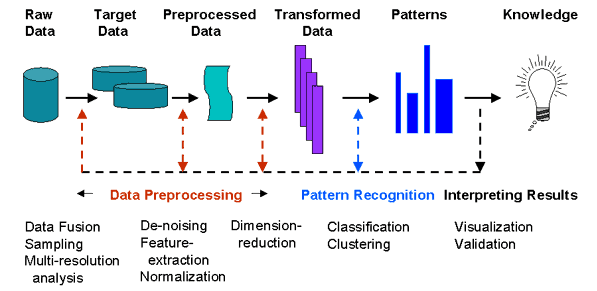
\includegraphics[scale=0.5]{data_mining_steps.png}
        \end{center}
    \end{frame}    
    
    \begin{frame}{Застосування}
        \begin{itemize}
            \item розпізнавання зображень, мови
            \item соціологія
            \item медицина
            \item маркетингові дослідження
        \end{itemize}
    \end{frame}
    
    
    \begin{frame}{Алгоритми}
        \begin{itemize}
            \item K-means
            \item DBSCAN
            \item UPGMA
            \item Neighbor-joining
        \end{itemize}
    \end{frame}
    
    
    \begin{frame}{Тестові дані}
        Тестування швидкодії алгоритмів проводилось на наборі даних розміром до 100000 об’єктів розмірності 8, 32 та 64.
        
        Кожен об’єкт вибірки --- вектор, всі компоненти якого лежать у проміжку $(-1; 1)$ та є випадковими величинами.
    \end{frame}
    
    
    \begin{frame}{Критерії оцінки ефективності}
        Ефективнсть реалізації кожного алгоритму оцінювалась в першу чергу за часом роботи.
        
        Для усіх алгоритмів час виконання одної ітерації не змінюється на протязі всього часу роботи, тому оцінювати можна зміни часу виконання ітерації.
    \end{frame}
    
    
    \begin{frame}{K-means --- оптимізації}
        \begin{center}
            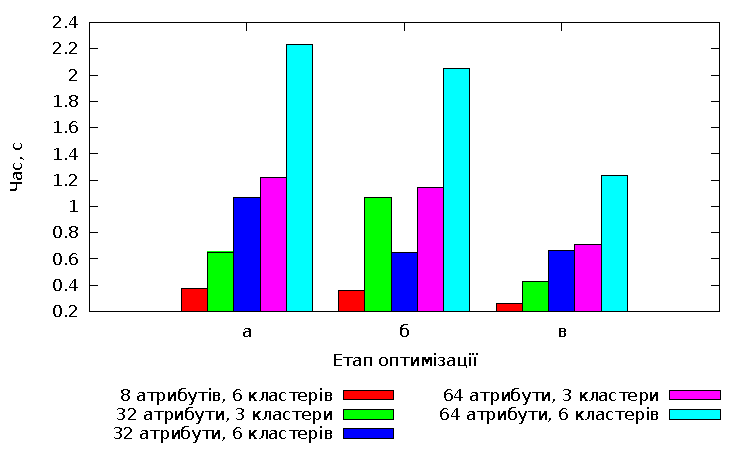
\includegraphics[scale=0.8]{kmeans_iteration_average.pdf}
        \end{center}
    \end{frame}
    
    
    \begin{frame}{K-means --- загальний час роботи}
        \begin{center}
            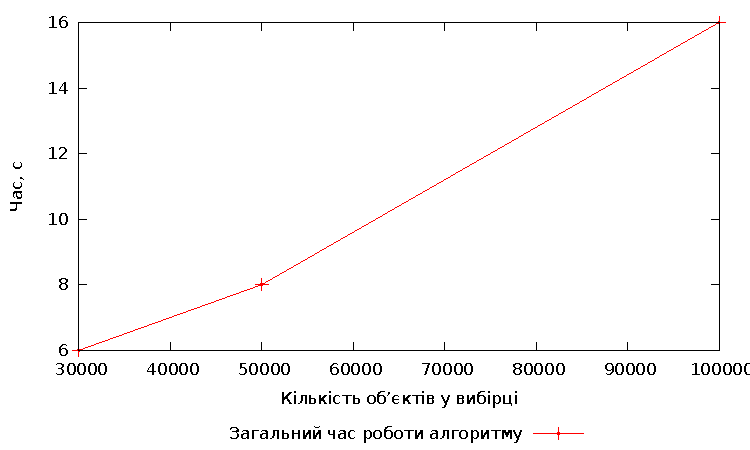
\includegraphics[scale=0.8]{kmeans_complexity.pdf}
        \end{center}
    \end{frame}
    
    
    \begin{frame}{DBSCAN --- оптимізації}
        \begin{center}
            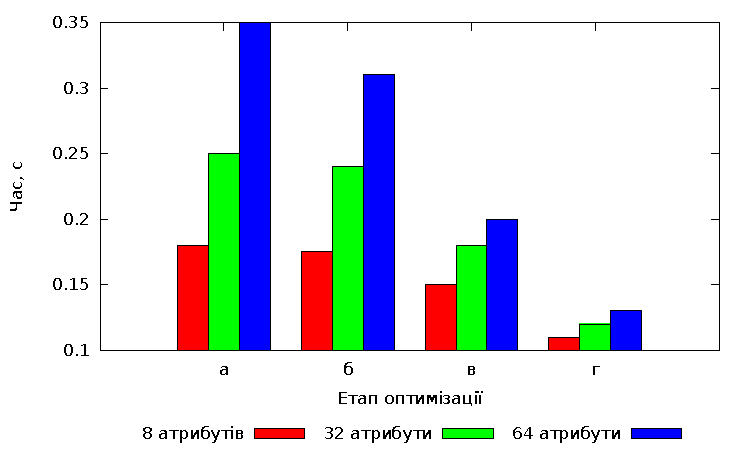
\includegraphics[scale=0.8]{dbscan_compare.pdf}
        \end{center}
    \end{frame}
    
    \begin{frame}{DBSCAN --- загальний час роботи}
        \begin{center}
            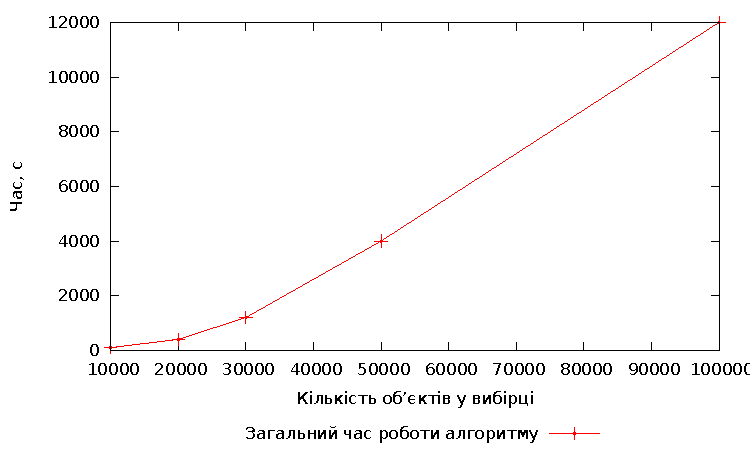
\includegraphics[scale=0.8]{dbscan_complexity.pdf}
        \end{center}
    \end{frame}    
    
        
    \begin{frame}{Neighbor-joining --- оптимізації}
        \begin{center}
            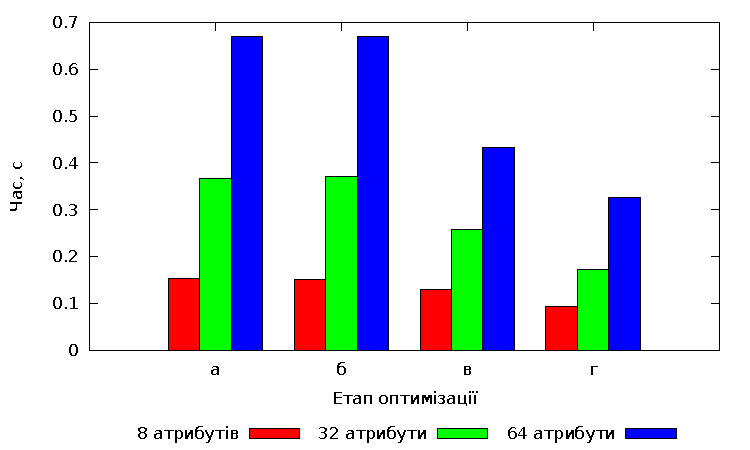
\includegraphics[scale=0.8]{nj_compare.pdf}
        \end{center}
    \end{frame}
    
    \begin{frame}{Neighbor-joining --- залежність часу одної ітерації від розміру вхідних даних}
        \begin{center}
            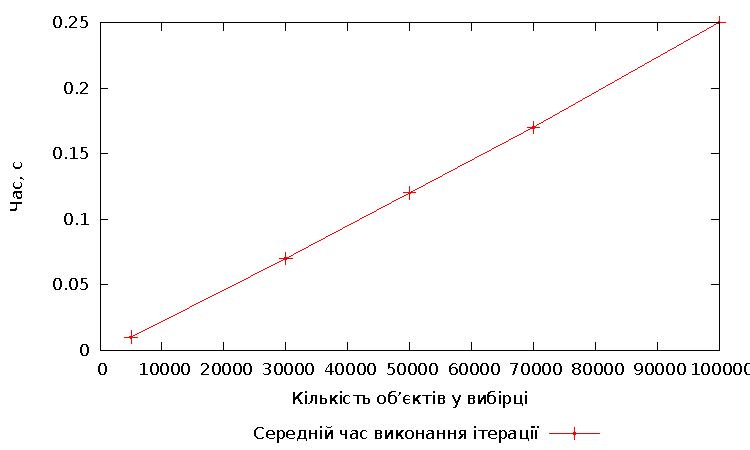
\includegraphics[scale=0.8]{nj_complexity.pdf}
        \end{center}
    \end{frame}
    
        
    \begin{frame}{Neighbor-joining --- оптимізації}
        \begin{center}
            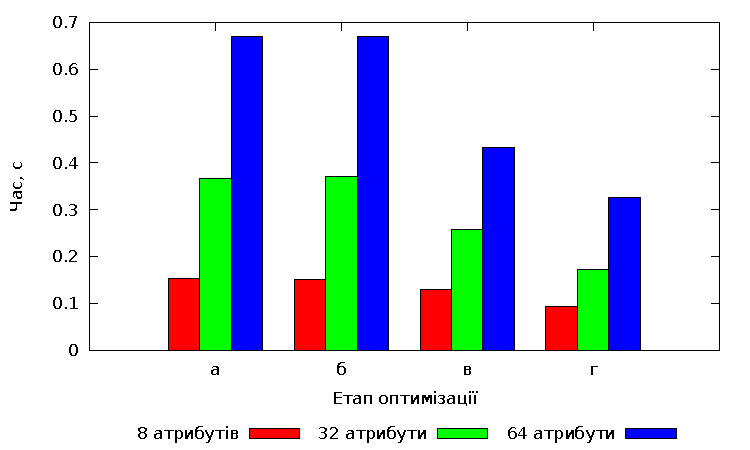
\includegraphics[scale=0.8]{nj_compare.pdf}
        \end{center}
    \end{frame}
    
    \begin{frame}{Neighbor-joining --- залежність часу одної ітерації від розміру вхідних даних}
        \begin{center}
            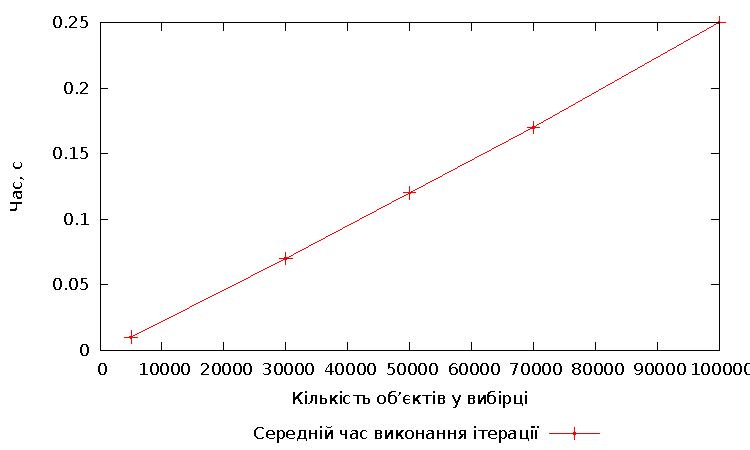
\includegraphics[scale=0.8]{nj_complexity.pdf}
        \end{center}
    \end{frame}
    
    
    \begin{frame}{UPGMA --- час ітерації}
        \begin{center}
            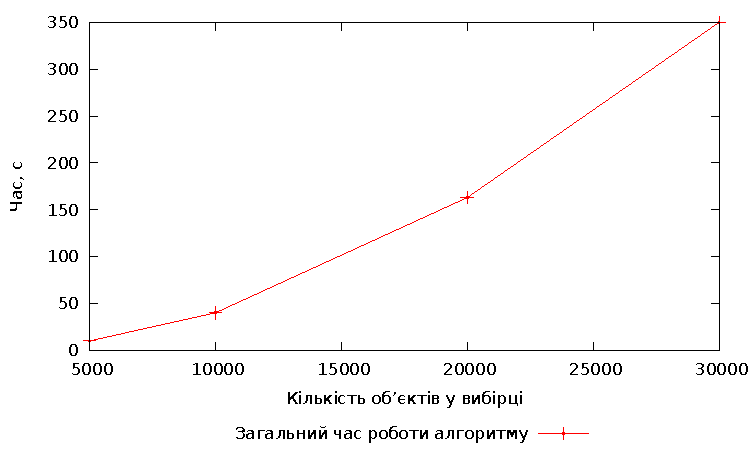
\includegraphics[scale=0.8]{upgma_real_complexity.pdf}
        \end{center}
    \end{frame}
    
\end{document}
